\documentclass{beamer}
\usetheme{Pittsburgh}
\usepackage{textpos}
\usepackage{lipsum}

%%%%%%%%%%%%%%%%%%%%%%%%%%%%%%%%%%%%%%%%%%%%%%%%%%%%%%%%%%%%%%%%%%%%%%%%%%%%%%%%
%%%%%%%%%%%%%%%%%%%%		Insert your variables here		%%%%%%%%%%%%%%%%%%%%
%%%%%%%%%%%%%%%%%%%%%%%%%%%%%%%%%%%%%%%%%%%%%%%%%%%%%%%%%%%%%%%%%%%%%%%%%%%%%%%%

\def\thetitle {\huge{Modeling of the shape of proteins from SAXS data}}		%Full title, displayed on first slide
\def\theshorttitle {Modeling of the shape of proteins} 			        %short title, displayed on all slides footers
\def\theauthor {Guillaume Bonamis}				%Full authors, displayed on first slide
\def\theshortauthor {Bonamis}					%Short authors, displayed on all slides footers
\def\thedate {Vendredi 4 Septembre}
\def\theinstitute {European Synchrotron Radiation Facility, Universit\'e Lille 1}%Full name of institute, displayed on first slide
\def\theshortinstitute {ESRF, Lille 1}			%Short name of institute, displayed on all slides footers

%%%%%%%%%%%%%%%%%%%%%%%%%%%%%%%%%%%%%%%%%%%%%%%%%%%%%%%%%%%%%%%%%%%%%%%%%%%%%%%%
%%%%%%%%%%%%%%%% ESRF beamer template from Pittsburgh theme %%%%%%%%%%%%%%%%%%%%

% Remove the navigation bar (but leave footer enabled)
\beamertemplatenavigationsymbolsempty%or \setbeamertemplate{navigation symbols}{}
%Template color
\definecolor{skyblue6}{RGB}{0,0,128}
\setbeamercolor{footline}{fg=skyblue6}
%\setbeamerfont{footline}{series=\bfseries}%bolderize footline text
%\setbeamercolor{title}{fg=whatever}
%\setbeamercolor{frametitle}{fg=whatever}
%\setbeamercolor{structure}{fg=whatever}

\title[\theshorttitle]{\thetitle}
\author[\theshortauthor]{

\includegraphics[scale=0.2]{ESRF_logo.png}
\\[20pt]
\theauthor
}
\institute[\theshortinstitute]{\theinstitute}
\date{\thedate}
\begin{document}
\begin{frame}
\maketitle
\end{frame}

%%%%%%%%%%%%%%%%%%%%%%%%%%%		Hearder, Footer	%%%%%%%%%%%%%%%%%%%%%%%%%%%%%%%%
%\setbeamertemplate{frametitle}[default][left]
\setbeamercolor{theheader}{fg=white,bg=skyblue6}
\setbeamertemplate{frametitle}{%
%\color{white}%\bfseries
\begin{beamercolorbox}[ht=2.5ex,dp=1ex,center]{theheader}
\usebeamerfont{title in head/foot}
%---Conditionally shows the section, subsection
\setbox0=\hbox{\secname\unskip}\ifdim\wd0=0pt\else%
\thesection{}.%
\fi
\setbox0=\hbox{\subsecname\unskip}\ifdim\wd0=0pt\else%
\thesubsection
\fi
%---
~\insertframetitle
\end{beamercolorbox}%
\par\vskip-6pt
}
%%%%
\addtobeamertemplate{footline}{}{%
\begin{textblock*}{600mm}(.68\textwidth,-1.1cm)

\includegraphics[scale=0.3]{ESRF_logo_bottom.png}
\end{textblock*}}
\setbeamerfont{footline}{size=\fontsize{5}{7}\selectfont}
\addtobeamertemplate{footline}{}{%
\begin{textblock*}{600mm}(.02\textwidth,-0.4cm)
\insertframenumber/\inserttotalframenumber
\hspace{3em}
\insertshorttitle
\hspace{3em}
\insertdate
\hspace{4em}
\insertshortauthor
\end{textblock*}}
%%%%%%%%%%%%%%%%%%%%	Further customization	%%%%%%%%%%%%%%%%%%%%%%%%%%%%%%%%
% Show plan at the beginning of each new section
\AtBeginSection[]
{
 \begin{frame}<beamer>[noframenumbering]
 \frametitle{Plan}
 \tableofcontents[currentsection]
 \end{frame}
}
\AtBeginSubsection[]{}
\setcounter{tocdepth}{2}
%%%%%%%%%%%%%%%%%%%%%%%%%%%%	Here we go	%%%%%%%%%%%%%%%%%%%%%%%%%%%%%%%%%%%%
\begin{frame}[noframenumbering]{Outline}
\tableofcontents
\end{frame}  


\section{SAXS et mod\'elisation structurale}
%-------------------------------------------
%----------------First part-----------------
%-------------------------------------------

\begin{frame}{G\'en\'eration de rayons X \`a l'ESRF}
%---------------------------------------------------
\vspace{-0.4cm}
\'electrons$\rightarrow$linac$\rightarrow$$1^{er}$ acc\'el\'erateur
$\rightarrow$ anneau de stockage (844m)

\vspace{0.4cm}
\begin{minipage}{0.70\linewidth}
    \begin{flushleft}
    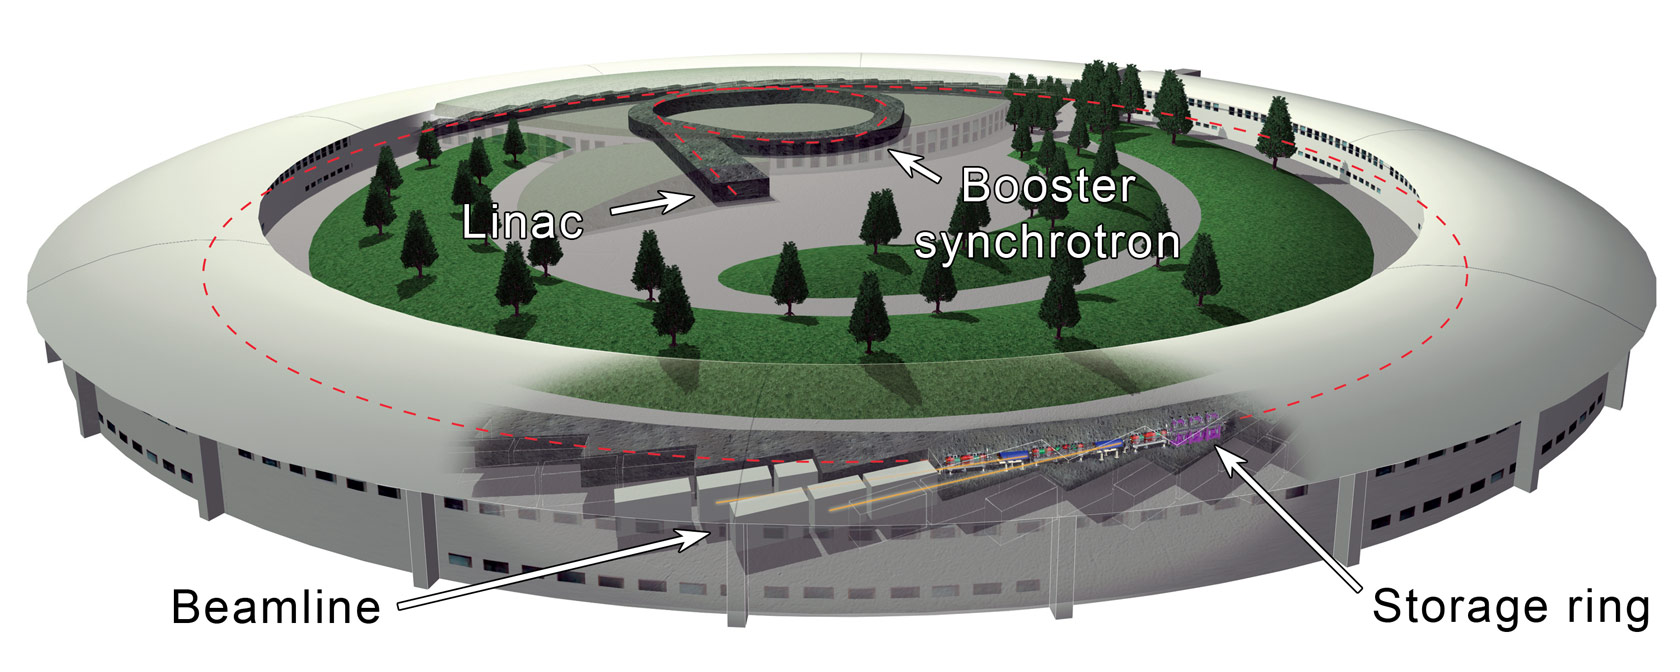
\includegraphics[scale=0.12]{synchrotron.png}
    \end{flushleft}
\end{minipage}
\fbox{\begin{minipage}{0.25\linewidth}
    \begin{flushleft}
    Rayons X :\\
    g\'en\'er\'es par le mouvement acc\'el\'er\'e d'\'electrons
    \end{flushleft}
\end{minipage}}

\vspace{0.4cm}
Dans l'anneau de stockage :\\
\begin{minipage}{0.45\linewidth}
    \begin{center}
    \vspace{-0.9cm}
    aimants de courbure\\
    \end{center}
\end{minipage}
\begin{minipage}{0.50\linewidth}
    $\Rightarrow$ trajectoire circulaire\\
    $\Rightarrow$ acc\'el\'eration \'electrons\\
    $\Rightarrow$ \'emission rayonnement
\end{minipage}

Sortie de l'anneau :\\
\begin{minipage}{0.45\linewidth}
    \begin{center}
    \vspace{-0.8cm}
    rayons X intenses\\
    \end{center}
\end{minipage}
\begin{minipage}{0.50\linewidth}
    $\Rightarrow$ entr\'ee dans une beamline (41)\\
    $\Rightarrow$ faisceau collimat\'e exploitable\\
\end{minipage}
\end{frame}

\begin{frame}{Exp\'eriences de SAXS sur BM 29}
BM 29 $\rightarrow$ ligne de lumi\`ere d\'edi\'ee \`a la BioSAXS\\
\begin{itemize}
  \item SAXS sur macromol\'ecules en solution
  \item acquisition figure de diffusion (2-d, symm\'etrique)
  \item int\'egration azimutale $\rightarrow$ \textbf{courbe de diffusion}
\end{itemize}

\begin{minipage}{\linewidth}
    \begin{flushleft}
    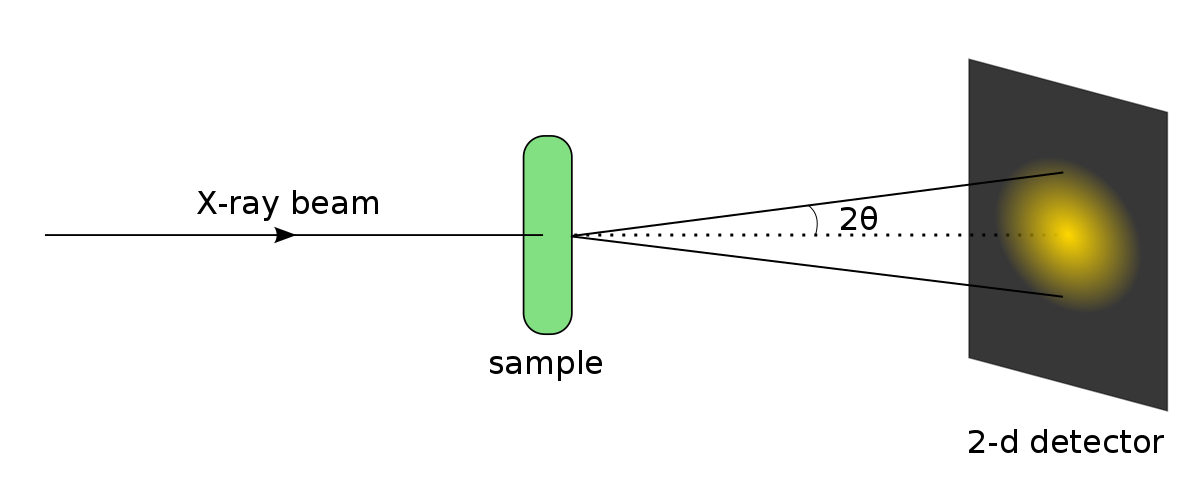
\includegraphics[scale=0.2]{schemaSAXS.png}
    \end{flushleft}
\end{minipage}

\underline{Objectif} : courbe de diffusion $\Rightarrow$ Mod\`ele 3-d 
de la structure de la macromol\'ecule
\end{frame}

\begin{frame}{Mod\'elisation structurale}
%----------------------------------------
Traitement des donn\'ees exp\'erimentales : syst\`eme \textbf{EDNA}
Programmes lanc\'es en s\'erie : 
%pipeline simplifiee pour presentation
\begin{enumerate}
  \item \textit{dammif} $\Rightarrow$ cr\'eation de $N$ mod\`eles 3-d 
    (Monte-carlo)
  \item \textit{supcomb} $\Rightarrow$ superposition des mod\'eles, \'ecarte 
    les "mauvais"
  \item \textit{damaver} $\Rightarrow$ moyenne des mod\`eles valides
  \item \textit{dammin} $\Rightarrow$ mod\`ele final, compatible avec la 
    courbe initiale
\end{enumerate}

\begin{minipage}{0.50\linewidth}
    mod\`eles 3-d basse r\'esolution (nm)\\
    structure $\rightarrow$ pseudo-atomes\\
    DAM = dummy-atoms model
\end{minipage}
\begin{minipage}{0.45\linewidth}
    \begin{center}
    \vspace{-0.3cm}
    \hspace{-0.4cm}
    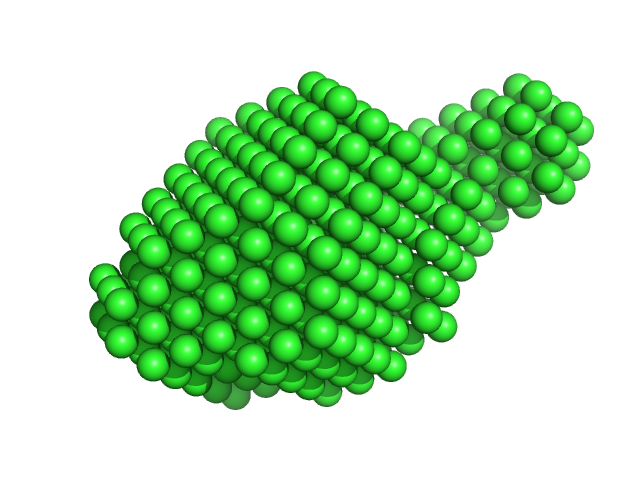
\includegraphics[scale=0.3]{model.png}
    \end{center}
\end{minipage}

\end{frame}

\section{Impl\'ementation}%titre a voir !!!
%-------------------------------------------
%----------------Second part----------------
%-------------------------------------------

\begin{frame}{Une autre diapo}
\lipsum[1]
\end{frame}


\section{Exemple}%titre a voir selon l'exemple presente !!!
%-------------------------------------------
%----------------Third part-----------------
%-------------------------------------------

\begin{frame}{Et encore une autre}
\lipsum[1]
\end{frame}

\end{document}
